\chapter{Background} \label{background}

The implementation of Skylab faced many design choices that shaped its fundamental development.  We describe and justify important major design choices here.

Skylab is built using Ruby on Rails, a well-known web development framework with a great support from a large community, used widely in the industries by companies like Twitter, Groupon, Bloomberg, Airbnb and many more\cite{citation1}. There are many reasons why we have chosen Ruby on Rails. Firstly, Ruby is clean, elegant and easy to read and readability and elegance of Ruby enables programmers to be more productive. Secondly, Ruby on Rails adopts many advanced industrial conventions and this enables contributors to have good exposure to programming in the industry. What is more, scaffolding and the contribution of many libraries (gems) by the Ruby community can significantly simplify programmers' work by saving time and effort of the development team from ``reinventing the wheel''.  The popularity and activeness in Ruby on Rails' community ensures that getting continuous support would be easy and many resources can also be available online. Last but not least, Ruby on Rails community has a favor for open source contribution which aligns well with the open source nature of Skylab.

For the selection of database, we used PostgreSQL. Part of the reason is that it is open source and quite mature, with good drivers available in many languages\cite{citation2}. Besides, we need full ACID (atomicity, consistency, isolation and durability) compliance for consistency of data and we do not need scalability to multiple servers in the foreseeable future\cite{citationACID}. And PostgreSQL has recently added implementation for rich data structures such as JSON which eases development\cite{citation3}.

Puma is the web server we have chosen for Skylab. Among common Ruby web servers such as Passenger, Unicorn, Rainbows!, Puma is considered to be fast and memory friendly according to online benchmarking\cite{citation4}. Puma is built for high-concurrency and speed and we observe that more developers are switching to Puma within the Rails community\cite{citation5}.

We have selected Nginx as our web (HTTP) server. Nginx has grown in popularity since its release due to its light-weight resource utilization and its ability to scale easily with low memory usage. It excels at serving static content quickly and is designed to pass dynamic requests off to other software that is better suited for those purposes\cite{citation6}. There are also some benchmarking results that indicate the superiority in Nginx handling concurrent access and of its small in-memory footprint\cite{citation7}.

A high-level overview of the architecture of Skylab is illustrated in Figure~\ref{fig:Skylabarch}. Incoming requests to server will first be forwarded to Puma worker processes by Nginx. After that the corresponding Skylab code in the Ruby on Rails framework will be executed. Where database access is required, PostgreSQL serves the data.

\begin{figure}[h]
  \centering
  \includegraphics[width=0.9\textwidth]{Images/Skylab_Arch.png}
  \caption{Architecture of Skylab}
  \label{fig:Skylabarch}
\end{figure}

\section{System design}

\subsection{MVC pattern in Ruby on Rails}

The basic MVC structure of Rails is shown in Figure~\ref{fig:RailsMVC}:

\begin{figure}[h]
  \centering
  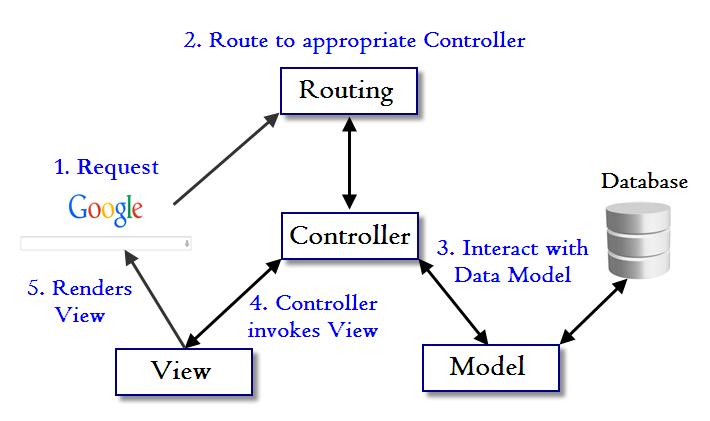
\includegraphics[width=0.85\textwidth]{Images/Rails_MVC.png}
  \caption{Illustration of how MCV works in Rails. Excerpted from \cite{citationMVC}}
  \label{fig:RailsMVC}
\end{figure}

After request is received by the Rails framework, the \textit{router} will look at the pattern of the requested URL path and send it to the corresponding method of the target \textit{controller} class. The \textit{controller} is supposed to query \textit{models} and gather necessary information for rendering the \textit{view}. Last but not least, the response will be sent back to user for viewing.

So the most fundamental component in this whole process is the \textit{model}, which stores all the business data. A proper model design can save a lot of trouble when it comes to writing controllers.

\subsection{Skylab Model Overview}

Figure~\ref{fig:SkylabER} (source available at \cite{citationERSource}) gives an overview of the current model design.

\begin{figure}[h]
  \centering
  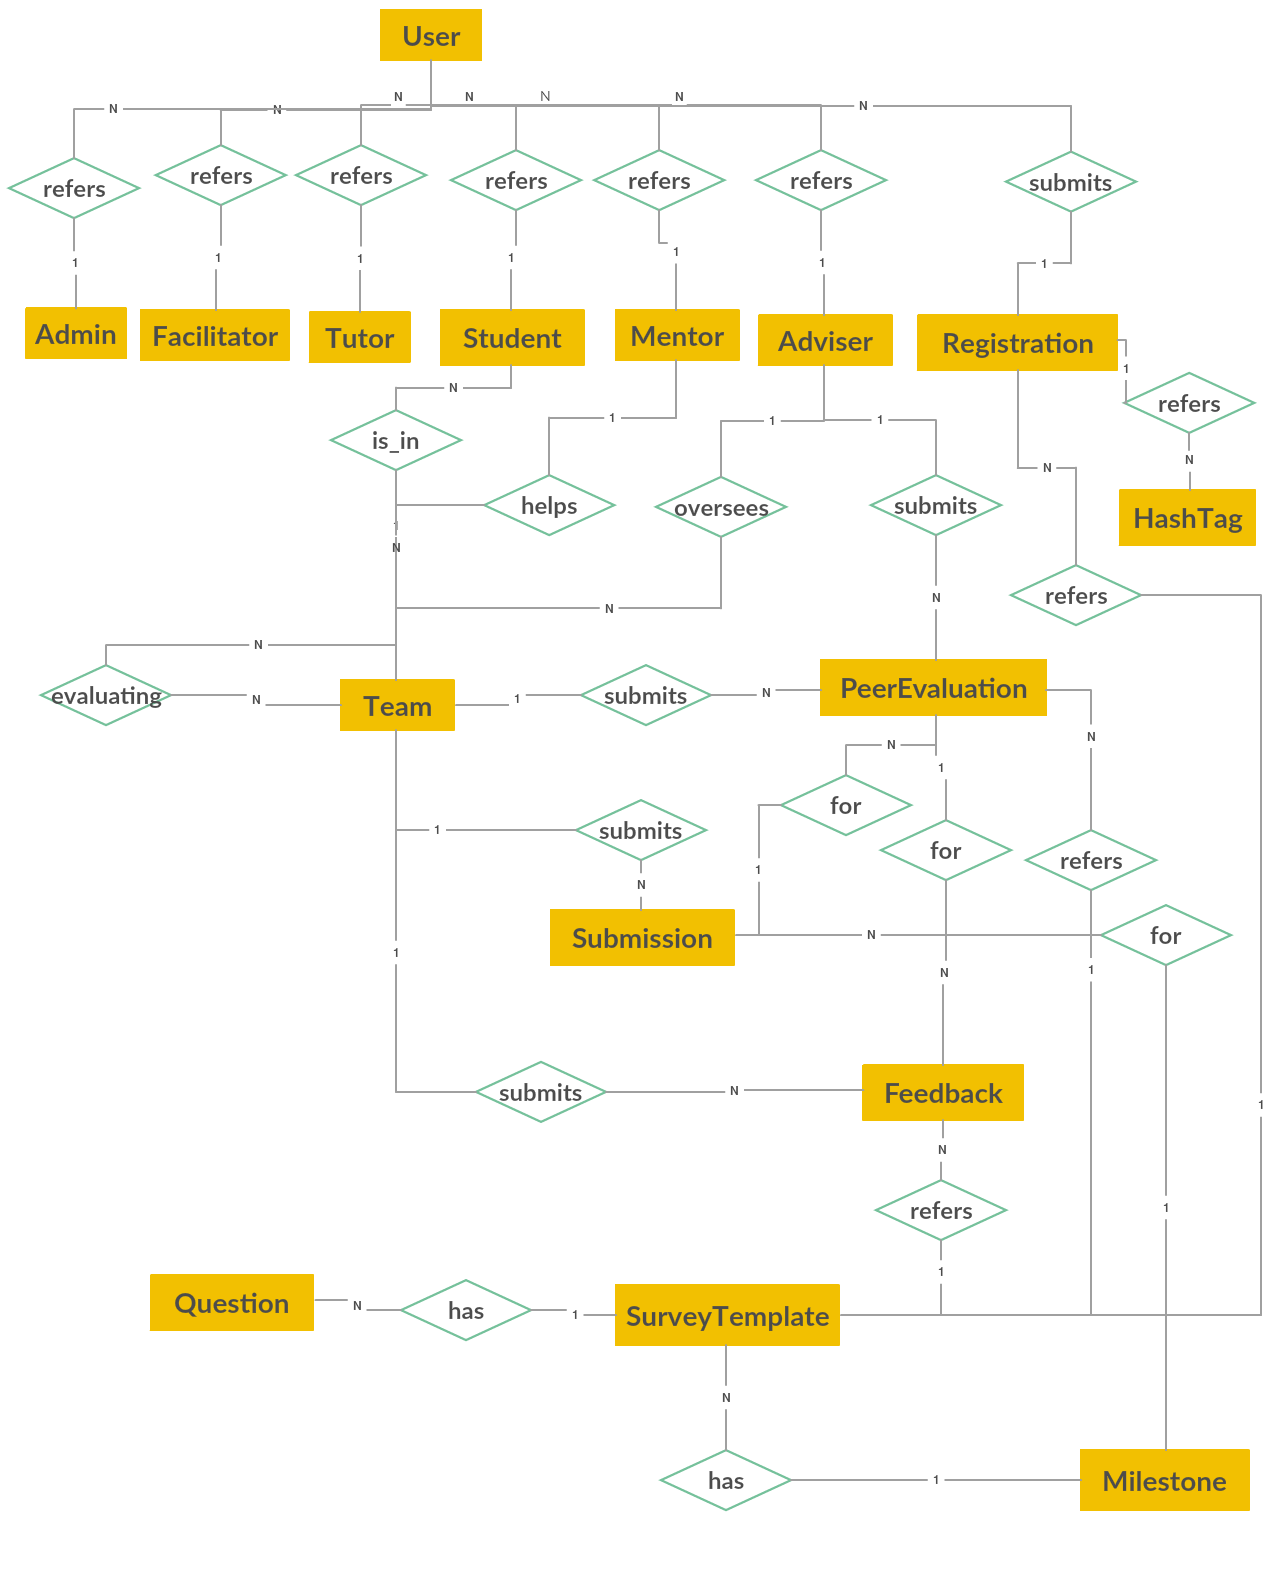
\includegraphics[width=\textwidth]{Images/Skylab_ER.png}
  \caption{Current ER diagram for Skylab}
  \label{fig:SkylabER}
\end{figure}

As is seen from the entity relation diagram shown in Figure~\ref{fig:SkylabER}, the users' basic information is captured in the \textit{User} model and each user may have one or more different roles such as \textit{Admin}, \textit{Student}, \textit{Adviser}, \textit{Mentor}, \textit{Tutor} and \textit{Facilitator}. Each user can have only one of any type of role in a cohort —-- meaning that if \textit{User} A is an \textit{Adviser} B for cohort 2015, then his/her adviser role for cohort 2015 will only be B (and of course he/she can also be a mentor, a tutor or another role type in cohort 2015). But for cohort 2016 if \textit{User} A is an adviser again, then it is another \textit{Adviser} role C. Roles like \textit{Facilitator}, \textit{Tutor} do not have practical meanings in the system but only for display in public staff page. \textit{Admin} is supposed to overlook manage everything in Skylab. The remaining roles, \textit{Adviser}, \textit{Mentors} and \textit{Student} are connected via different relationships.

Each student has a \textit{Team} and a team has an \textit{Adviser} and a \textit{Mentor} (optional). A group of teams under the same adviser is called an \textit{Evaluation Group} and evaluating relationships will be assigned from team to team in the same \textit{Evaluation Group}. Each team will create \textit{Submissions} to \textit{Milestones} to report their progress and their adviser and assigned evaluator teams will submit \textit{PeerEvaluations} to the team's \textit{Submissions}. After receiving \textit{PeerEvaluation} from evaluator teams and adviser, the team need to provide \textit{Feedback} to rate the helpness of those \textit{PeerEvaluations}.

Before Orbital officially starts, interested students need to register in Skylab first. A \textit{Registration} will be created to record information about the student and his/her interested topics of project in the summer for recommending potential teammates if they do not have a partner in mind at the time of registration.

\textit{PeerEvaluation}, \textit{Feedback} and \textit{Registration} can be considered as \textit{Surveys}. Basically a \textit{Survey} contains some instructions and consists of questions to be answered. So in Skylab, a \textit{SurveyTemplate} would record information like instructions to students and have many \textit{Questions} to form a \textit{Survey}. Responses of \textit{Survey} would be stored in \textit{PeerEvaluation}, \textit{Feedback} and \textit{Registration}.

\subsection{Overview of Controllers in Skylab}

Controllers will query models to get information needed to present views or make modifications to models if requested. Therefore they are crucial in powering a Rails application and in Skylab we have well-defined controllers to carry out different tasks. A class diagram of all controllers in Skylab is shown in Figure~\ref{fig:SkylabControllers}.

\begin{figure}[h]
  \centering
  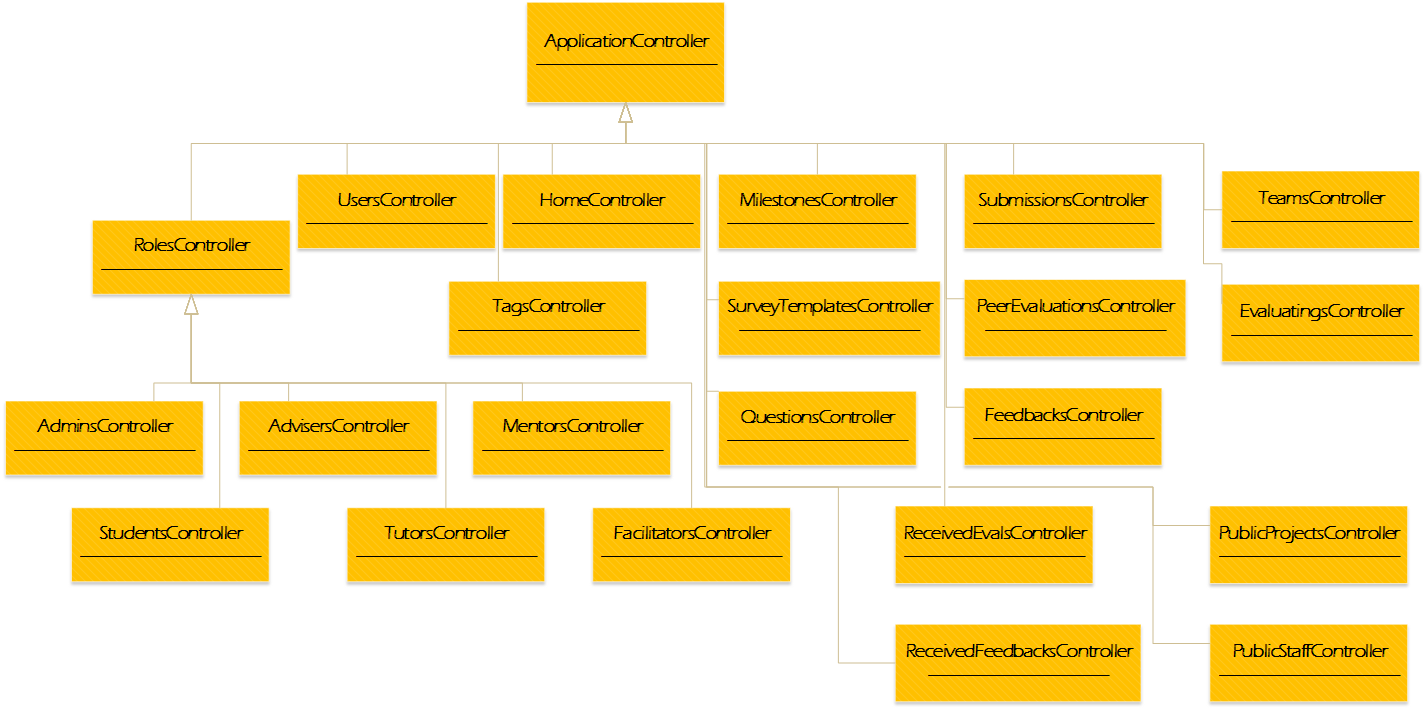
\includegraphics[width=\textwidth]{Images/Skylab_Controllers.png}
  \caption{Current Class diagram of controllers in Skylab}
  \label{fig:SkylabControllers}
\end{figure}

\textit{ApplicationController} is the base of all other controllers. Utility methods such as access control, page title and handling of exceptions are included in \textit{ApplicationController} and it also includes auxiliary modules such as \textit{CohortHelper} to enrich its functionality. \textit{RolesController} is the base class of all roles' controller classes: \textit{AdminsController}, \textit{AdvisersController}, \textit{MentorsController}, \textit{StudentsController}, \textit{FacilitatorsController} and \textit{TutorsController}. These roles share quite a lot in common so they will share request processing methods and they will override data related methods or provide some handlers for special cases. Other controllers are as follows:

\begin{itemize}
  \item \textbf{HomeController}: serves home page to user only.
  \item \textbf{UsersController}: manages listing, creation, editing and display of users and also includes functionality for admin to masquerade as any user, for new users to register as students in Orbital.
  \item \textbf{TagsController}: lists tags based on specified filters.
  \item \textbf{MilestonesController}: handles listing, creation, editing and display of milestones.
  \item \textbf{SurveyTemplatesController}: handles listing, creation, editing and display of survey templates and also serves as interface for editing of questions belonging to current survey templates. 
  \item \textbf{QuestionsController}: manages Ajax requests to create, edit or delete a question.
  \item \textbf{SubmissionsController}: manages creation, editing and display of submissions by students.
  \item \textbf{PeerEvaluationsController}: handles creation, editing and display of peer evaluations from evaluator teams or advisers to evaluated teams.
  \item \textbf{FeedbacksController}: manages creation, editing and display of feedback from evaluated team to evaluator teams or advisers.
  \item \textbf{ReceivedEvalsController}: compiles a set of received peer evaluations for a team in one milestone.
  \item \textbf{ReceivedFeedbacksConroller}: compiles a set of received feedback for a team or an adviser in one milestone.
  \item \textbf{PublicProjectsController}: serves completed teams' projects to the public.
  \item \textbf{PublicStaffController}: serves staff of Orbital program to the public.
  \item \textbf{TeamsController}: manages listing, creation, editing and display of teams.
  \item \textbf{EvaluatingsController}: handles listing, creation, editing and display of evaluating relation among teams.
\end{itemize}

Controllers manage a collection of \textit{resources} in Skylab, meaning that each controller is managing one model class, to facilitate higher cohesion. If there is a necessary dependency on other models --- for example, SurveyTemplate will manage questions belonging to current SurveyTemplate --- the requests will be handled by Ajax requests to separate concerns.

Skylab follows the Ruby on Rails convention for controller classes. A basic controller that manages a collection has the following structure illustrated in Figure~\ref{fig:SkylabSampleController}.

\begin{figure}[h]
  \centering
  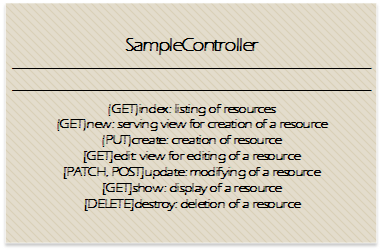
\includegraphics[width=0.5\textwidth]{Images/Skylab_Sample_Controller.png}
  \caption{Sample controller class in Skylab}
  \label{fig:SkylabSampleController}
\end{figure}

These methods —-- \textit{index}, \textit{new}, \textit{create}, \textit{edit}, \textit{update}, \textit{show} and \textit{destroy} —-- have included all the basic actions to be done with a collection of resources. Following this convention makes controller class design in Skylab consistent and easy to read, and also aligns well with the goal of creating a more human-readable RESTful URL design.

\section{Development / source code management process}

GitHub flow is used in Skylab's development process. It is simple but agile enough for project management. Skylab is a web application for which releases of new versions do not require any user action. Each release can be deployed to server without users noticing it. This flow is quite different from traditional Git flow, which is far more complex and puts a lot of focus on each release\cite{citation8}. In fact, in GitHub flow, each commit on master branch should be releasable and continuous deployment is recommended\cite{citation8}. Each feature will be developed on a feature branch and once the feature is ready, a pull request is created against master. After code review and running test suite, pull requests are merged into the master branch and is then ready for deployment (Figure~\ref{fig:GithubFlow}).

\begin{figure}[h]
  \centering
  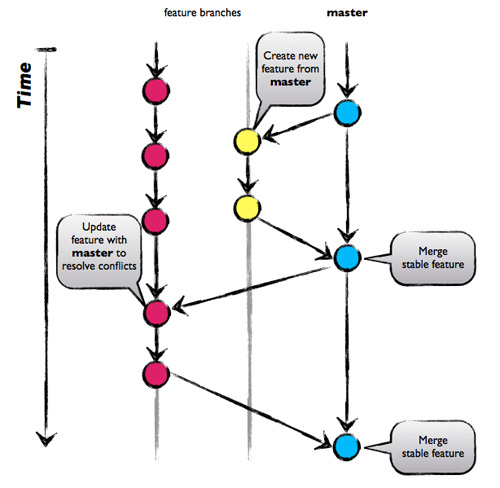
\includegraphics[width=0.85\textwidth]{Images/Github_Flow_Branching_Model.png}
  \caption{Branching diagram for GitHub Flow. Excerpted from \cite{citation8}}
  \label{fig:GithubFlow}
\end{figure}

By using GitHub flow and services such as Travis as the continuous integration service\cite{citationtravis}, CodeClimate as the code quality monitoring service\cite{citationcodeclimate}, we keep the development of Skylab agile and fast. The use of GitHub flow enables Skylab to deployed regularly, which is essential for timely improvement of user experience\cite{citation9}.
